\documentclass[aspectratio=169]{beamer}

% ---------------------------------------------------------------------------
% Theme
% ---------------------------------------------------------------------------
\usetheme{Madrid}
\usecolortheme{whale}
\setbeamertemplate{navigation symbols}{}
\setbeamercovered{transparent}

\usepackage[utf8]{inputenc}
\usepackage[T1]{fontenc}
\usepackage{amsmath, amssymb}
\usepackage{graphicx}
\usepackage{booktabs}
\usepackage{tikz}
\usetikzlibrary{shapes, arrows.meta, positioning, fit}
\usepackage{hyperref}
\hypersetup{colorlinks=true, linkcolor=, urlcolor=blue}

% ---------------------------------------------------------------------------
% Title
% ---------------------------------------------------------------------------
\title[Roofline \& Kernel Fusion of Window Attention]{%
  Roofline Analysis \& Kernel Fusion of Window Attention on Apple M4}
\subtitle{Project Proposal}
\author{Anurag Dhiman}
\institute{}
\date{\today}

\begin{document}

% =============================================================================
\begin{frame}
  \titlepage
\end{frame}

\begin{frame}{Outline}
  \tableofcontents
\end{frame}

% =============================================================================
\section{Introduction}
% =============================================================================

\begin{frame}{Motivation}
  \begin{itemize}
    \item Vision Transformers are increasingly deployed on \textbf{edge and consumer hardware}
      (phones, tablets, laptops), where inference latency and memory traffic matter as much
      as accuracy.
    \item \textbf{TinyViT} \cite{wu2022tinyvit} reduces compute by replacing global self-attention
      with \textbf{local window attention} (as in Swin Transformer~\cite{liu2021swin}), typically
      over small $7\times7$ windows.
    \item Apple Silicon GPUs (e.g.\ the M4) expose a \textbf{unified-memory} architecture accessed
      through PyTorch's MPS backend or Apple's own \textbf{MLX} framework.
    \item Small-window attention involves many \emph{small} tensor operations: reshaping,
      permutation, transposition, and repeated kernel dispatches --- exactly the regime where
      per-op overhead can dominate raw FLOPs.
  \end{itemize}
\end{frame}

\begin{frame}{The Problem with FLOPs Alone}
  \begin{columns}[T]
    \begin{column}{0.55\textwidth}
      \begin{itemize}
        \item Window attention has low nominal FLOP counts, so it is often assumed to be
          ``free'' relative to convolutions and MLPs.
        \item In practice, implementations add:
        \begin{itemize}
          \item tensor reshape / permute / view operations,
          \item intermediate buffer materialization,
          \item many small, separately-dispatched GPU kernels.
        \end{itemize}
        \item On a \textbf{unified-memory} GPU, these introduce real memory traffic and
          dispatch latency that FLOP counting cannot see.
      \end{itemize}
    \end{column}
    \begin{column}{0.45\textwidth}
      \centering
      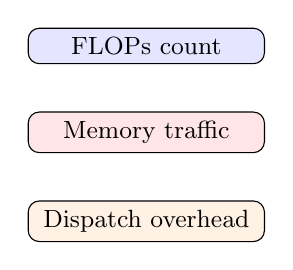
\begin{tikzpicture}[node distance=6mm, every node/.style={font=\small}]
        \node[draw, rounded corners, fill=blue!10, minimum width=3.0cm] (a) {FLOPs count};
        \node[draw, rounded corners, fill=red!10, minimum width=3.0cm, below=of a] (b) {Memory traffic};
        \node[draw, rounded corners, fill=orange!10, minimum width=3.0cm, below=of b] (c) {Dispatch overhead};
      \end{tikzpicture}
      \\[2mm]
      {\small \Large ?} \\[1mm]
      {\small What actually determines latency?}
    \end{column}
  \end{columns}
\end{frame}

\begin{frame}{Why a Roofline Model}
  \begin{itemize}
    \item The \textbf{Roofline model}~\cite{williams2009roofline} relates achievable performance
      to \emph{arithmetic intensity} (FLOPs per byte moved):
    \[
      P(I) = \min\bigl(P_{\max},\; B_{\max} \cdot I\bigr), \qquad
      I_{\text{ridge}} = \frac{P_{\max}}{B_{\max}}
    \]
    \item Classical roofline analysis explains \textbf{compute-bound} vs.\ \textbf{memory-bound}
      behavior --- but \textbf{not} kernel-launch / dispatch overhead, which can dominate for
      many small operations.
    \item This project builds an \textbf{empirical} (measured, not vendor-spec) roofline for the
      Apple M4 GPU, maps TinyViT's actual stages onto it, and separately characterizes dispatch
      overhead.
  \end{itemize}
\end{frame}

% =============================================================================
\section{Research Questions}
% =============================================================================

\begin{frame}{Primary Research Question}
  \begin{block}{}
    \centering
    \Large
    How much of TinyViT's inference latency on Apple M4 is caused by \textbf{low arithmetic
    intensity}, \textbf{memory movement}, and \textbf{kernel/dispatch overhead} in window-based
    attention --- and how much can be reduced through \textbf{kernel fusion}?
  \end{block}
\end{frame}

\begin{frame}{Sub-Questions}
  \begin{enumerate}
    \item What is the empirically measured compute throughput ($P_{\max}$) and memory bandwidth
      ($B_{\max}$) of the Apple M4 GPU, and where does window attention sit relative to the
      resulting roofline?
    \item Which sub-stages of window attention (QKV projection, attention score, softmax,
      attention--value product, output projection, layout transforms) are compute-bound,
      memory-bound, or dispatch-bound?
    \item How does latency scale with \textbf{window size}, \textbf{embedding dimension},
      \textbf{number of windows}, and \textbf{batch size}?
    \item Does kernel fusion (via MLX/Metal) measurably reduce intermediate materialization,
      memory traffic, and kernel-launch count relative to the standard PyTorch/MPS
      implementation?
    \item Do any such gains hold up under \textbf{correctness} constraints (numerical
      equivalence) and translate into \textbf{end-to-end} inference speedup?
  \end{enumerate}
\end{frame}

% =============================================================================
\section{Methodology}
% =============================================================================

\begin{frame}{Overview: Eight-Phase Experimental Pipeline}
  \begin{center}
  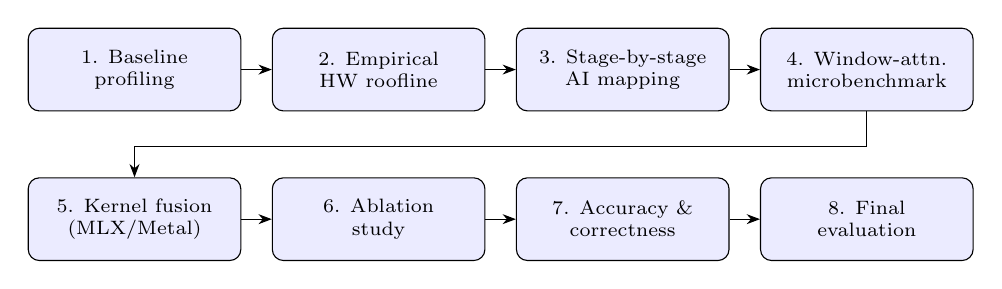
\begin{tikzpicture}[
      phase/.style={draw, rounded corners, fill=blue!8, minimum width=2.7cm, minimum height=1.05cm, align=center, font=\scriptsize},
      >=Stealth
    ]
    % Row 1: phases 1-4, left to right, on a 3.1cm horizontal grid, y = 0
    \node[phase] (p1) at (0*3.1cm, 0)  {1. Baseline\\profiling};
    \node[phase] (p2) at (1*3.1cm, 0)  {2. Empirical\\HW roofline};
    \node[phase] (p3) at (2*3.1cm, 0)  {3. Stage-by-stage\\AI mapping};
    \node[phase] (p4) at (3*3.1cm, 0)  {4. Window-attn.\\microbenchmark};
    % Row 2: phases 5-8, left to right, y = -1.9cm, same x grid so arrows are short
    \node[phase] (p5) at (0*3.1cm, -1.9cm) {5. Kernel fusion\\(MLX/Metal)};
    \node[phase] (p6) at (1*3.1cm, -1.9cm) {6. Ablation\\study};
    \node[phase] (p7) at (2*3.1cm, -1.9cm) {7. Accuracy \&\\correctness};
    \node[phase] (p8) at (3*3.1cm, -1.9cm) {8. Final\\evaluation};

    \draw[->] (p1) -- (p2);
    \draw[->] (p2) -- (p3);
    \draw[->] (p3) -- (p4);
    \draw[->] (p4.south) -- ++(0,-0.45cm) -| (p5.north);
    \draw[->] (p5) -- (p6);
    \draw[->] (p6) -- (p7);
    \draw[->] (p7) -- (p8);
  \end{tikzpicture}
  \end{center}
  Each phase is independently runnable and produces its own measured artifacts (no step depends
  on unverified assumptions from a previous step).
\end{frame}

\begin{frame}{Phase 1: Baseline Profiling}
  \begin{itemize}
    \item Profile the \textbf{standard, unmodified} pretrained TinyViT forward pass --- no
      hand-tuning --- so the baseline reflects real default performance.
    \item Collected via \texttt{torch.profiler} on the MPS backend, supplemented by
      Metal/MPS-level tracing where PyTorch-level profiling is insufficient:
    \begin{itemize}
      \item total and per-block latency,
      \item op-level dispatch-time breakdown (by category: conv, linear, attention, layout, \ldots),
      \item kernel-launch / op-count proxy,
      \item peak memory usage, input/output tensor sizes.
    \end{itemize}
    \item \textbf{Caveat to validate:} MPS executes asynchronously, so naive CPU-side timing
      measures \emph{dispatch} time, not GPU execution time --- this distinction must be verified
      before it is used for roofline placement.
  \end{itemize}
\end{frame}

\begin{frame}{Phase 2--3: Empirical Roofline \& Arithmetic Intensity}
  \begin{columns}[T]
    \begin{column}{0.5\textwidth}
      \textbf{Empirical hardware roofline}
      \begin{itemize}
        \item Measure $P_{\max}$ via a matmul-size sweep.
        \item Measure $B_{\max}$ via a memory-bound
          elementwise-op size sweep.
        \item Compute the ridge point $I_{\text{ridge}} = P_{\max}/B_{\max}$.
        \item Measured, not taken from vendor marketing specs.
      \end{itemize}
    \end{column}
    \begin{column}{0.5\textwidth}
      \textbf{Per-stage arithmetic intensity}
      \begin{itemize}
        \item Closed-form FLOPs / bytes-moved for: convolution blocks, QKV projection, attention
          score, softmax, attention--value product, output projection, layout transforms.
        \item Applied to each block's \emph{actual} shapes (not a single hand-derived case).
        \item Each stage is plotted at $(AI, P_{\text{achieved}})$ on the measured roofline.
      \end{itemize}
    \end{column}
  \end{columns}
\end{frame}

\begin{frame}{Phase 4: Window-Attention Microbenchmark}
  \begin{itemize}
    \item Controlled sweep, isolating window attention as a standalone operator, varying:
    \begin{itemize}
      \item window size ($4\times4$, $7\times7$, $14\times14$),
      \item embedding dimension,
      \item number of windows,
      \item batch size.
    \end{itemize}
    \item Decompose total attention latency:
    \[
      T_{\text{attention}} = T_{\text{QKV}} + T_{\text{reshape}} + T_{\text{attn}} +
        T_{\text{softmax}} + T_{\text{proj}} + T_{\text{dispatch}}
    \]
    \item Goal: determine whether small-window attention genuinely suffers from a
      small-GEMM / dispatch-overhead problem, and how that overhead scales with each axis.
  \end{itemize}
\end{frame}

\begin{frame}{Phase 5: Kernel-Fusion Implementation}
  \begin{itemize}
    \item \textbf{Baseline path:}
    \[
      X \rightarrow QKV \rightarrow \text{window partition} \rightarrow QK^\top \rightarrow
      \text{softmax} \rightarrow AV \rightarrow \text{window reverse} \rightarrow \text{proj}
    \]
    \item \textbf{Fused path} (MLX/Metal), minimizing intermediate materialization:
    \[
      X \;\longrightarrow\; \boxed{\text{Fused Window Attention}} \;\longrightarrow\; Y
    \]
    \item Specifically targets reduction of: intermediate tensors, global-memory
      reads/writes, tensor-layout conversions, and kernel launches.
    \item Every fused variant is gated by a \textbf{numerical-equivalence check}
      (max-abs-difference, cosine similarity) against the standard baseline before its speed is
      trusted.
  \end{itemize}
\end{frame}

\begin{frame}{Phase 6: Ablation Study}
  \begin{table}
    \centering
    \small
    \begin{tabular}{ll}
      \toprule
      \textbf{Configuration} & \textbf{Purpose} \\
      \midrule
      PyTorch/MPS baseline        & Original, unmodified implementation \\
      Optimized PyTorch           & Compiler-level optimization (\texttt{torch.compile}) \\
      Fused attention (MLX/Metal) & Test kernel fusion \\
      Different window sizes      & Test locality / parallelism \\
      Different batch sizes       & Test utilization \\
      Different embedding dims    & Test arithmetic intensity \\
      \bottomrule
    \end{tabular}
  \end{table}
  \vspace{2mm}
  Each arm is compared against the \emph{same} standard baseline under the \emph{same}
  measurement methodology.
\end{frame}

\begin{frame}{Phase 7--8: Correctness, Accuracy \& Final Evaluation}
  \begin{itemize}
    \item \textbf{Correctness:} numerical equivalence at the operator level, and end-to-end
      top-1 / top-5 accuracy on real ImageNet-1k images, comparing every implementation's
      predictions against the standard baseline's.
    \item \textbf{Final metrics reported together:}
    \begin{itemize}
      \item Speedup $= T_{\text{baseline}} / T_{\text{optimized}}$
      \item latency reduction, kernel-launch reduction, estimated memory-traffic reduction
      \item effective TFLOP/s, effective bandwidth, arithmetic intensity achieved
      \item end-to-end TinyViT inference speedup
      \item accuracy difference (correctness-gated: speed is only reported for implementations
        verified to preserve predictions)
    \end{itemize}
  \end{itemize}
\end{frame}

% =============================================================================
\section{Expected Contributions}
% =============================================================================

\begin{frame}{Expected Contributions}
  \begin{enumerate}
    \item An \textbf{empirical Roofline model} for the Apple M4 GPU (measured $P_{\max}$,
      $B_{\max}$, ridge point), reusable beyond this project.
    \item A \textbf{stage-by-stage Roofline characterization} of TinyViT's window attention,
      identifying which sub-operations are compute-, memory-, or dispatch-bound.
    \item A \textbf{working kernel-fusion implementation} of window attention via MLX/Metal,
      verified for numerical correctness against the standard baseline.
    \item A \textbf{before/after memory-traffic and kernel-launch analysis} quantifying what
      fusion does and does not change.
    \item An \textbf{end-to-end inference benchmark} reporting speedup (or its absence) together
      with accuracy, so that any claimed gain is both real and safe.
  \end{enumerate}
\end{frame}

\begin{frame}{Framing the Contribution}
  \begin{block}{Key scientific contribution}
    \centering
    Characterizing and reducing the compute, memory, and dispatch inefficiencies of small-window
    attention on Apple Silicon through empirical Roofline analysis and kernel fusion.
  \end{block}
  \vspace{4mm}
  \begin{itemize}
    \item The project is designed to report a \textbf{true} result either way: if fusion does
      not yield a net speedup for a given configuration, that is itself a finding about where the
      standard implementation is already efficient --- and about where the \emph{real} bottleneck
      lies.
    \item All benchmarking methodology (warm-up, synchronization, isolation between
      configurations) will be validated before being trusted, since GPU-level timing on a
      unified-memory, asynchronously-executing backend is easy to measure incorrectly.
  \end{itemize}
\end{frame}

% =============================================================================
\section{References}
% =============================================================================

\begin{frame}[allowframebreaks]{References}
  \small
  \begin{thebibliography}{99}

  \bibitem{wu2022tinyvit}
    K.~Wu, J.~Zhang, H.~Peng, M.~Liu, B.~Xiao, J.~Fu, and L.~Yuan.
    \newblock TinyViT: Fast Pretraining Distillation for Small Vision Transformers.
    \newblock In \emph{European Conference on Computer Vision (ECCV)}, 2022.

  \bibitem{liu2021swin}
    Z.~Liu, Y.~Lin, Y.~Cao, H.~Hu, Y.~Wei, Z.~Zhang, S.~Lin, and B.~Guo.
    \newblock Swin Transformer: Hierarchical Vision Transformer using Shifted Windows.
    \newblock In \emph{IEEE/CVF International Conference on Computer Vision (ICCV)}, 2021.

  \bibitem{dosovitskiy2021vit}
    A.~Dosovitskiy, L.~Beyer, A.~Kolesnikov, D.~Weissenborn, X.~Zhai, T.~Unterthiner,
    M.~Dehghani, M.~Minderer, G.~Heigold, S.~Gelly, J.~Uszkoreit, and N.~Houlsby.
    \newblock An Image is Worth 16x16 Words: Transformers for Image Recognition at Scale.
    \newblock In \emph{International Conference on Learning Representations (ICLR)}, 2021.

  \bibitem{williams2009roofline}
    S.~Williams, A.~Waterman, and D.~Patterson.
    \newblock Roofline: An Insightful Visual Performance Model for Multicore Architectures.
    \newblock \emph{Communications of the ACM}, 52(4):65--76, 2009.

  \bibitem{paszke2019pytorch}
    A.~Paszke et al.
    \newblock PyTorch: An Imperative Style, High-Performance Deep Learning Library.
    \newblock In \emph{Advances in Neural Information Processing Systems (NeurIPS)}, 2019.

  \bibitem{mlx2023}
    Apple Machine Learning Research.
    \newblock \emph{MLX: An array framework for Apple silicon}.
    \newblock \url{https://github.com/ml-explore/mlx}, 2023.

  \bibitem{apple_mps}
    Apple Inc.
    \newblock \emph{Metal Performance Shaders / PyTorch MPS Backend Documentation}.
    \newblock \url{https://developer.apple.com/metal/pytorch/}.

  \bibitem{vaswani2017attention}
    A.~Vaswani, N.~Shazeer, N.~Parmar, J.~Uszkoreit, L.~Jones, A.~N.~Gomez, {\L}.~Kaiser, and
    I.~Polosukhin.
    \newblock Attention Is All You Need.
    \newblock In \emph{Advances in Neural Information Processing Systems (NeurIPS)}, 2017.

  \end{thebibliography}
\end{frame}

\begin{frame}
  \centering
  \Huge Thank you
  \\[4mm]
  \Large Questions?
\end{frame}

\end{document}
